\documentclass[10pt,a4paper]{article}
\usepackage[utf8]{inputenc}
\usepackage[T1]{fontenc}
\usepackage{amsmath}
\usepackage{amsthm}
\usepackage{amssymb}
\usepackage{graphicx}
\usepackage{mathtools}
\usepackage[ruled,vlined,linesnumbered]{algorithm2e}
\usepackage[left=2.50cm, right=2.50cm, top=2.0cm, bottom=2.0cm]{geometry}


\makeatother
\DeclareMathOperator*{\argmin}{argmin}
\DeclareMathOperator*{\Max}{\text{max}}
\DeclareMathOperator*{\E}{\mathbb{E}}
\newcommand{\Ei}[1]{\mathbb{E}_{#1}}
\DeclareMathOperator*{\Eik}{\mathbb{E}_{\mathit{i_k}}}
\DeclareMathOperator*{\Eikplus}{\mathbb{E}_{\mathit{i_{k+1}}}}
\newcommand{\Eiplus}[1]{\mathbb{E}_{i_{#1}}}
\DeclareMathOperator*{\LC}{\text{\textup{LC}}^1}
\DeclareMathOperator*{\grad}{\mathit{\nabla \!f}}
\DeclareMathOperator*{\argmax}{arg\;max}
\DeclareMathOperator*{\gradik}{\mathit{\nabla\!\fik}}
\DeclareMathOperator*{\Lmax}{\mathit{L_{max}}}
\newcommand{\R}{\mathbb{R}}
\newcommand{\st}{\text{s.t.} \;\;\;}
\newcommand{\Rn}{\mathbb{R}^n}
\newcommand{\ikplus}{i_{k+1}}
\newcommand{\wrefi}[2]{w_{r(#1, i_{#2})}}
\newcommand{\wref}[1]{\wrefi{#1}{#1}}
\newcommand{\fik}{f_{i_k}}
\newcommand{\fikofwstar}{\fik(w^*)}
\newcommand{\fofwstar}{f(w^*)}
\newcommand{\fii}[1]{f_{i_{#1}}}
\newcommand{\fikplus}{f_{i_{k+1}}}
\newcommand{\fiplus}[1]{f_{i_{#1}}}
\newcommand{\fimax}{f_i^{\text{max}}}
\newcommand{\fikmax}{\fik^{\text{max}}}
\newcommand{\bmax}{b_{\text{max}}}
\newcommand{\fmax}{f^{\text{max}}}
\newcommand{\fmaxk}[1]{f_{i_{#1}}^{\text{max}}}
\newcommand{\Lik}{L_{i_k}}
\newcommand{\Cik}{C_{i_k}}
\newcommand{\deltak}{\delta^{l_k}}
\newcommand{\deltakplus}{\delta^{l_k+1}}
\newcommand{\deltakminus}{\delta^{l_k-1}}
\newcommand{\etatilde}{\tilde{\eta}_{k,0}}
\newcommand{\muik}{\mu_{i_k}}
\newcommand{\etamax}{\eta^{\text{max}}}
\newcommand{\etamaxx}{\bar{\eta}^{\text{max}}}
\newcommand{\etamin}{\eta^{\text{min}}}
\newcommand{\etaminn}{\bar{\eta}^{\text{min}}}
\newcommand{\minimum}[2]{\min \left\{ #1, #2 \right \} }
\newcommand{\maximum}[2]{\max \left\{ #1, #2 \right \} }
\newcommand{\W}[1]{{\scriptscriptstyle W #1}}
\newcommand{\gradi}[1]{\nabla f_{i_{#1}} (w_{i_{#1}}) }
\makeatletter

\newtheorem{assumption}{Assumption}
\newtheorem{lemma}{Lemma}
\newtheorem{proposition}{Proposition}
\newtheorem{theorem}{Theorem}
\newtheorem{corollary}{Corollary}
\newtheorem{remark}{Remark}


\newcommand{\imgS}{.26}
\newcommand{\dir}{exp1/}
\newcommand{\model}{mlp}
\newcommand{\modelname}{mlp}


\newcommand{\mlp}{{\texttt{mnist|mlp}}}
\newcommand{\res}{{\texttt{cifar10|resnet34}}}
\newcommand{\dense}{{\texttt{cifar10|densenet121}}}
\newcommand{\ress}{{\texttt{cifar100|resnet34}}}
\newcommand{\denses}{{\texttt{cifar100|densenet121}}}
\newcommand{\fashion}{{\texttt{fashion|effb1}}}
\newcommand{\svhn}{{\texttt{svhn|wrn}}}
\newcommand{\wiki}{{\texttt{wiki2|encoder}}}
\newcommand{\ptb}{{\texttt{ptb|xl}}}
\newcommand{\mushrooms}{{\texttt{mushrooms}}}
\newcommand{\rcvone}{{\texttt{rcv1}}}
\newcommand{\ijcnn}{{\texttt{ijcnn}}}
\newcommand{\weighta}{{\texttt{w8a}}}

\title{Continuous Optimization}
\author{Chapter 2: Gradient Descent}
\date{}
\begin{document}
	\maketitle
	\section{Descent Direction Methods}
	\noindent In this chapter we consider the unconstrained minimization problem
	\begin{equation*}
		\min_{x\in\Rn} \;\; f(x).
	\end{equation*}
The iterative algorithms that we will consider in this chapter take the form
\begin{equation*}
	x_{k+1} = x_k +t_k d_k \quad k=0,1, \dots,
\end{equation*}
where $d_k$ is the so-called direction and $t_k$ is the step size. We will limit ourselves to descent
directions, whose definition is now given.
\begin{definition}
	Let $f:\Rn\to\R$ with $f\in\C(\Rn)$ and $x\in \Rn$. A vector $0\neq d\in \Rn$ is called a descent direction of $f$ at $x$ if the directional derivative $f'(x,d)$ is negative, i.e., 
	\begin{equation*}
		f'(x,d)= \grad(x)^T d < 0.
	\end{equation*}
\end{definition}
\noindent In particular, by taking small enough steps, descent directions lead to a decrease of the objective function.
\begin{lemma}[descent property of descent directions]
	Let $f:\Rn\to\R$ with $f\in\C(\Rn)$ and let $x\in \Rn$. Suppose that $d$ is a descent direction of $f$ at $x$. Then, there exists $\epsilon>0$ such that 
	\begin{equation*}
		f(x+td) < f(x) \quad \forall \, t \in (0,\epsilon].
	\end{equation*} 
\end{lemma}
\begin{proof}
	Since $f'(x,d)<0$, it follows from the definition of the directional derivative that 
	\begin{equation*}
		\lim_{t\to 0^+}\frac{f(x+td)-f(x)}{t} = f'(x,d) <0.
	\end{equation*}
Therefore, there exists an $\epsilon>0$ such that 
\begin{equation*}
	\frac{f(x+td)-f(x)}{t}<0,
\end{equation*}
for any $t\in(0,\epsilon)$
\end{proof}
\begin{algorithm}[H]\label{alg}
	\caption{Schematic Descent Directions Method}
	
	\KwIn{$x_0\in \Rn$}
	
	$k = 0$
	
	\While{Termination criterion is not satisfied}{
				
			Pick a descent direction $d_k$
			
			Find a step size $t_k$ satisfying $f(x_k+t_kd_k)<f(x_k)$
			
			$x_{k+1} = x_k+t_kd_k$
			
			$k = k+1$
		}
\end{algorithm}
\noindent Various choices are still unspecified: which direction to take, how to select the step size, what termination criterion to use.
\section{Gradient Method}
\noindent The most important choice in the algorithm above concerns the selection of the descent direction. One obvious choice is to pick the steepest (normalized) direction, i.e., $d_k =-\grad(x_k)/||\grad(x_k)||$. In fact, this direction minimizes the directional derivatives between all normalized directions. 
\begin{lemma}
	Let $f:\Rn\to\R$ with $f\in\C(\Rn)$ and let $x\in\Rn$ be non-stationary (i.e., $\grad(x)\neq0$). Then the optimal solution of the problem
	\begin{equation*}
		\begin{split}
			\min \;\; &f'(x,d),\\
			\st& ||d||=1.
		\end{split}
	\end{equation*}
is $d=-\frac{\grad(x)}{||d||}$.
\end{lemma}
\begin{proof}
	As $f\in \C(\Rn)$ and by Cauchy-Schwarz, we have 
	\begin{equation*}
		f'(x,d)=\grad(x)^Td \geq -||\grad(x)||\cdot ||d|| = -||\grad(x)||.
	\end{equation*}
Thus, $-||\grad(x)||$ is a lower bound for the optimal value of the problem. On the other hand, by plugging  $d = -\grad(x)/||\grad(x)||$ in the objective function we get 
\begin{equation*}
	f'\left(x,-\frac{\grad(x)}{||\grad(x)||}\right)=-\grad(x)^T\left(\frac{\grad(x)}{||\grad(x)||}\right)= -||\grad(x)||,
\end{equation*}
and we thus come to the conclusion that the lower bound is attained at $d=-\frac{\grad(x)}{||d||}$.
\end{proof}
\noindent Thus, the gradient method selects $d_k = -\grad(x_k)$ which is obviously a descent direction, i.e., 
\begin{equation*}
\grad(x_k)^Td_k = -\grad(x_k)^T\grad(x_k) = -||\grad(x)||^2.
\end{equation*}
\noindent To define an implementable method, the second important choice we have to make is the selection of the step size $t$. In particular, this will be clearer once we provide the Descent Lemma below, which require the gradient to be Lipschitz continuous. 
\begin{definition}[Lipschitz Continuous Gradient]
	$\grad(x)$ is said to be Lipschitz continuous if 
	\begin{equation*}
		|| \grad(x) -\grad(y)|| \leq L ||x-y|| \quad \forall x,y \in \Rn.
	\end{equation*}
The class of functions with Lipschitz continuous gradient with constant $L$ is denoted by $\LC(\Rn)$.
\end{definition}
\begin{theorem}
	Let $f\in\Cii(\Rn)$. Then the following two claims are equivalent:
	\begin{itemize}
		\item[(a)] $f\in \LC(\Rn)$
		\item[(b)] $||\hess(x)||\leq L \quad \forall x\in \Rn$.
	\end{itemize}
\begin{proof}
	$(b)\Rightarrow (a)$. Suppose that $||\hess(x)||\leq L \quad \forall x\in \Rn$. By the fundamental theorem of calculus we have $\forall x,y \in \Rn$
	\begin{equation*}
		\begin{split}
			\grad(y)=\grad(x) + \int_{0}^{1} \hess(x+t(y-x)) (y-x) dt = \grad(x) + \left(\int_{0}^{1} \hess(x+t(y-x)) dt  \right) \cdot (y-x)
		\end{split}
	\end{equation*}
Thus, 
\begin{equation*}
	\begin{split}
		||\grad(y)-\grad(x)|| &= \left \| \left(\int_{0}^{1} \hess(x+t(y-x)) dt  \right) \cdot (y-x)\right \|\\
		&\leq \left\|\int_{0}^{1} \hess(x+t(y-x)) dt  \right\| \cdot \|(y-x) \|\\
		& \leq \left(\int_{0}^{1}|| \hess(x+t(y-x))|| dt  \right)\cdot \|(y-x) \|\\
		& \leq L \|(y-x) \|
	\end{split}
\end{equation*}
	$(a)\Rightarrow (b)$. Exercise.
\end{proof}
\end{theorem}
\begin{lemma}[Descent Lemma (prequel)] Let $f\in \LC(\Rn)$. Then for any $x,y \in \Rn$
	\begin{equation*}
		f(y) \leq f(x) + \grad(x)^T(y-x) + \frac{L}{2} \|x-y\|^2.
	\end{equation*}
\end{lemma}
\begin{proof}
From the fundamental theorem of calculus and differentiability of $f$ we have 
\begin{equation*}
	\begin{split}
		f (y) & = f(x) + \int_{0}^{1} \grad((1-t)x + t y)^T\! (y-x) \; dt\\
		& = f(x) + \int_{0}^{1} \grad((1-t)x + t y)^T\! (y-x) - \grad(x)^T(y-x) \; dt + \grad(x)^T(y-x)\\ 
		&\leq f(x) + \int_{0}^{1} \| \grad((1-t)x + t y) - \grad(x)\|\! \cdot\! \|y-x\| \; dt + \grad(x)^T(y-x)\\  
		& \leq f(x) + \int_{0}^{1} L \| t(y-x) \|\! \cdot\! \|y-x\| \; dt + \grad(x)^T(y-x)\\
		& = f(x) + L\|y-x\|^2 \cdot \frac{t^2}{2} \Big|_0^1 + \grad(x)^T(y-x)\\
		& = f(x) + \grad(x)^T(y-x) + \frac{L}{2} \|y-x\|^2,
	\end{split}
\end{equation*}
where the second inequality follows from the Lipschitz continuity of $\grad$.
\end{proof}
\begin{lemma}[Descent Lemma]\label{lemma:descent} Let $f\in \LC(\Rn)$. Then for any $x \in \Rn$ and $t>0$
	\begin{equation*}
		f(x) - f(x-t\grad(x)) \geq t (1-\frac{Lt}{2}) \| \grad(x)\|^2.
	\end{equation*}
\end{lemma}
\begin{proof}
	The result simply follows by applying the descent lemma (prequel) on $x$ and $y=x-\grad(x)$
	\begin{equation*}
		f(x-t\grad(x))\leq f(x) -t ||\grad(x)\|^2 + \frac{Lt^2}{2} \|\grad(x)\|^2 = f(x) - t (1-\frac{Lt}{2}) \| \grad(x)\|^2
	\end{equation*}
\end{proof}
\noindent In particular, this holds for $x=x_k$ and $x_{k+1} = x_k -\grad(x_k)$,
\begin{equation*}
	f(x_k) - f(x_{k+1}) \geq t (1-\frac{Lt}{2}) \| \grad(x_k)\|^2,
\end{equation*}
which in turns implies that if we select $t\in (0,\frac{2}{L})$ we ensure a decrease of the objective function at each iteration. In particular, if we want to achieve the largest guarantee bound on the decrease, then we seek the maximum of $t (1-\frac{Lt}{2})$ w.r.t. $t$, which is attained at $t=\frac{1}{L}$ with a decrease that becomes
\begin{equation}\label{eq:decrease}
	f(x_k) - f(x_{k+1}) \geq \frac{1}{2L} \| \grad(x_k)\|^2.
\end{equation}
At this point we can write down the Gradient Method in terms of an implementable algorithm.

\begin{algorithm}[H]\label{gd}
	\caption{Gradient Descent (GD) Method}
	
	\KwIn{Pick $x_0\in \Rn$ arbitrarly, chose $\epsilon>0$ (e.g., $10^{-4}$).}
	
	$k = 0$
	
	\While{$\|\grad(x_k)\|> \epsilon$}{
		
		$x_{k+1} = x_k - \frac{1}{L} \grad(x_k)$
		
		$k = k+1$
	}
\end{algorithm}
\noindent Let us now prove convergence for GD, in particular that $\grad(x_k)$ goes to zero.
\begin{theorem}[Convergence of GD]\label{thm:GD_convergence}
	Let $f\in \LC(\Rn)$ and let $\{x_k\}_k$ be a sequence generated by Algorithm \ref{alg} for solving $\min_{x\in\Rn}\;f(x)$. Assume that $f$ is bounded below over $\Rn$, i.e., there exists $m\in \R$ such that $f(x)>m \;\; \forall\, x\in \Rn$. Then we have the following
	\begin{itemize}
		\item[(a)] The sequence $\{f(x_k)\}_k$ is nonincreasing. In addition, for any $k\geq 0$, $f(x_{k+1}) < f(x_k)$ unless $\grad(x_k)=0$.
		\item[(b)] $\grad(x_k) \to 0$ as $k\to \infty$.
	\end{itemize}
\begin{proof}
	(a) directly follows from \eqref{eq:decrease}, as $f(x_{k+1}) < f(x_k)$ and the equality $f(x_{k+1}) = f(x_k)$ only holds when $\grad(x_k)=0$.
	(b) Since the sequence $\{f(x_k)\}_k$ is nonincreasing and bounded from below, it converges. Thus, $f(x_k) - f(x_{k+1}) \to 0$ as $k\to \infty$, which combined with \eqref{eq:decrease} implies that $\|\grad(x_k)\|\to 0$ as $k\to \infty$.  
\end{proof}
\end{theorem}
\noindent Moreover, we can provide the rate of convergence of GD.
\begin{theorem}[Rate of Convergence of GD]
	Under the setting of Theorem \ref{thm:GD_convergence}, let $f^*$ be the limit of the convergent sequence $\{f(x_k)\}_k$. Then for any $T=0,1, \dots$
	\begin{equation*}
		\min_{k=0,1,\dots, T} \| \grad(x_k) \|\leq \sqrt{\frac{L (f(x_0) -f^*)}{T+1}}
	\end{equation*}
\end{theorem}
\begin{proof}
	Summing the inequality \eqref{eq:decrease} over $k=0, 1, \dots, T$, we obtain 
	\begin{equation*}
		f(x_0) - f(x_{T+1}) = \frac{1}{L}\sum_{k=0}^{T} \|\grad(x_k)\|^2\geq \frac{T+1}{L} \min_{k=0,1,\dots, T} \| \grad(x_k)\|^2
	\end{equation*}
which concludes the proof.
\end{proof}
%TODO: how to remove the min?
%\bibliographystyle{plain}
%\bibliography{../biblio}
\subsection{Line search methods}
The gradient method as defined above can only be employed when we know or we can compute the Lipschitz constant $L$, on the other hand, we would like to have a general method that can be applied on any unconstrained optimization problem. An alternative for selecting the step size is provided by line search methods. Consider a direction $d_k$, one option would be to exactly minimize along the direction $d_k$, i.e., \textbf{exact line search}
\begin{equation*}
	t_k \in \argmin_{t>0} f(x_k+t d_k).
\end{equation*}
However, this approach is not always viable and even when it is, it might be costly. Another option is instead that of accepting a step that will make the function value decrease "sufficiently", namely to apply an \textbf{inexact line search}. In particular, the first line search proposed in the literature is called Armijo line search \cite{armijo66a} and it requires the following
\begin{equation}\label{eq:armijo}
	f(x_k +t_k d_k) \leq f(x_k) + \alpha t_k\grad(x_k)^Td_k.
\end{equation}
Notice that if we define $\phi(t)=f(x_k+td_k)$ we can rewrite the inequality above as
\begin{equation*}
\phi(t_k) \leq \phi(0) + \alpha t_k \phi'(0) \qquad \with \alpha \in (0,1).
\end{equation*}
As depicted in Figure 1, the condition requires that the new function value $\phi(t_k)$ stays below the line passing for $(0,\phi(0))$ and with $\alpha\phi'(0)$ as inclination. Notice that as $\phi'(0)<0$ and $\alpha<1$, the line $y=\phi(0) +\alpha t_k \phi'(0)$ is not as inclined as the tangent in 0. The way for selecting a step $t_k$ that satisfies \eqref{eq:armijo} is suggested by the figure.
\begin{figure}
	\centering
	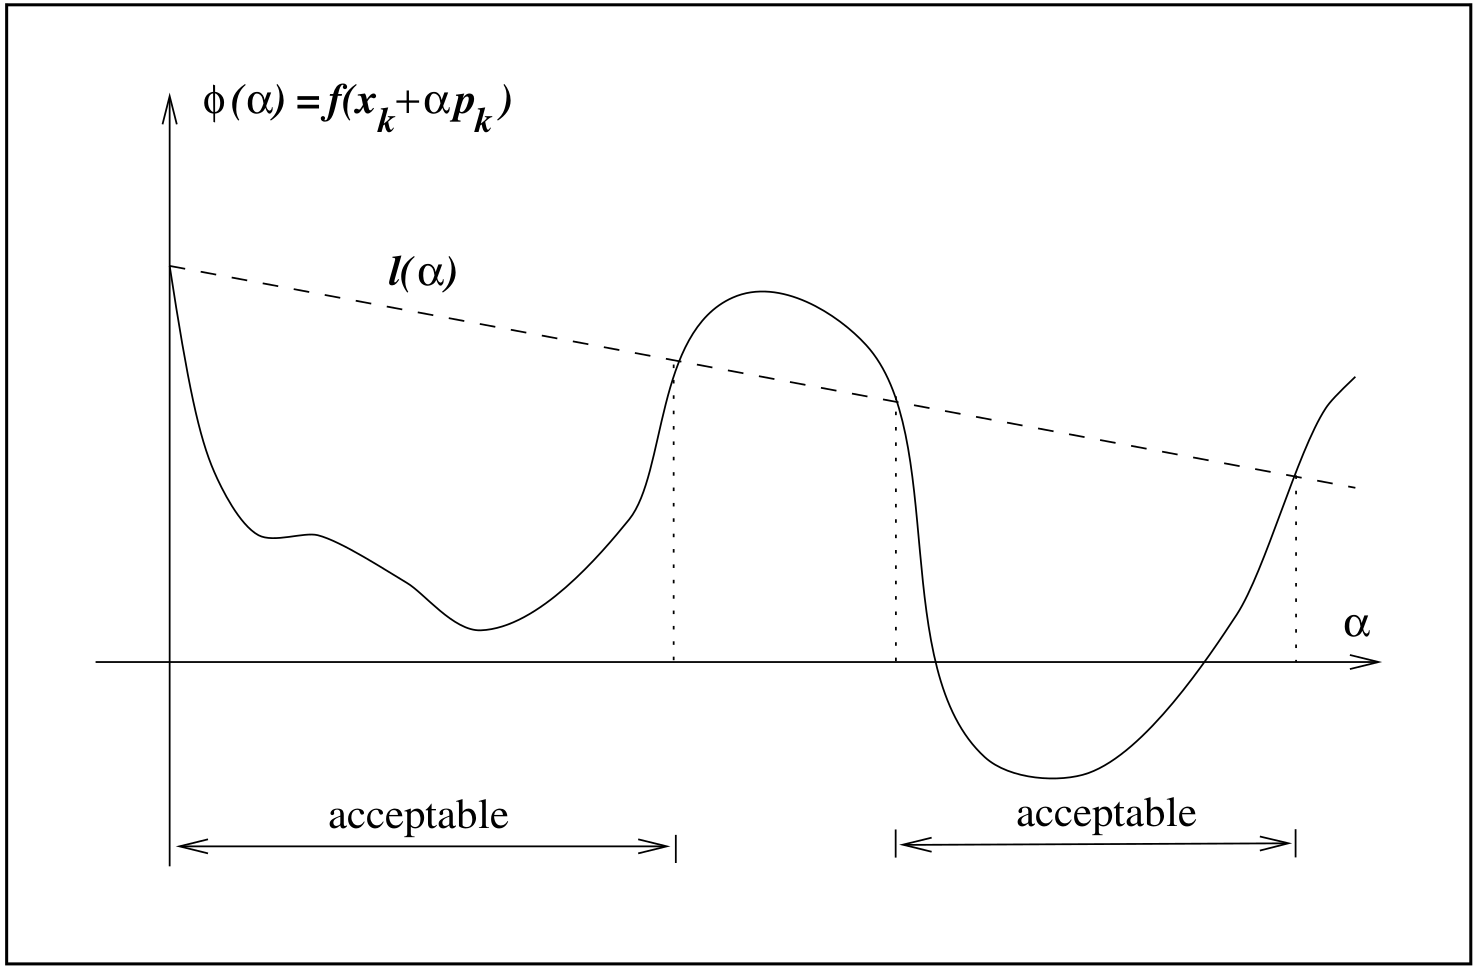
\includegraphics[width=0.5\linewidth]{lines}
	\caption{The figure represents the Armijo line search condition (the notation in this figure is different from the text, replace $\alpha$ in the figure with $t$ from the text.)}
\end{figure}
In particular, the method is called backtracking and it is described below.
\begin{algorithm}[H]\label{alg:armijo}
	\caption{Backtracking on Armijo line search}
	
	\KwIn{Pick $s>0$, $\alpha,\beta \in(0,1)$.}
	
	$i=0$	
	
	\Do{$f(x_k +t_k d_k) > f(x_k) + \alpha t_k \grad(x_k)^Td_k$}{
		
		$t_k = s \beta^i$
		
		$i=i+1$
	}
	
\end{algorithm}
\noindent Let us first show that this method terminates in a finite amount of steps
\begin{lemma} \label{lemma:finite_termination}
	Let $f\in \LC(\Rn)$, $x\in \Rn$ and $d\in \Rn$ be a descent direction. Then Algorithm \ref{alg:armijo} terminates in a finite amount of steps with a $t_k>0$ that satisfies \eqref{eq:armijo}. Moreover, one of the following holds
	\begin{itemize}
		\item[(a)] $t_k=s$
		\item[(b)] $t_k\leq \beta s$ such that $f(x_k +\frac{t_k}{\beta} d_k) > f(x_k) + \alpha \frac{t_k}{\beta} \grad(x_k)^Td_k$
	\end{itemize}
Consequently, with $d_k = -\grad(x_k)$ we get $t_k \geq \min \left\{s, \frac{2(1-\alpha)\beta}{L} \right \}$.
\end{lemma}
\begin{proof}
	Let us first prove that the algorithm terminates in a finite amount of steps. By contradiction there are no finite value of $i$ for which \eqref{eq:armijo} is satisfied, that is 
	\begin{equation*}
		\frac{f(x_k +s \beta^i d_k)- f(x_k)}{s \beta^i} > \alpha \grad(x_k)^Td_k.
	\end{equation*}
Given $\beta<1$ we have that $\lim_{i\to \infty} \beta^i =0$ and thus, with $i\to \infty$ the LHS of the inequality above is the directional derivative of $f$ along $d_k$. In particular, we get
\begin{equation*}
	\grad(x_k)^Td_k \geq \alpha\grad(x_k)^Td_k,
\end{equation*}
which is a contradiction, as $\grad(x_k)^Td_k<0$ and $\alpha <1$.
Following the steps of the algorithm, either the first guess $s$ is accepted or $t_k\leq s\beta$. In the second case, given $t_k$ the outcome of the algorithm, the step size before the last backtracking ($\frac{t_k}{\beta}$) was surely not accepted, from which (b) follows.
\par Now, we can replace $\frac{t_k}{\beta}$ in Lemma \ref{lemma:descent} with $x=x_k$ to get
\begin{equation*}
	f(x_k) - f(x_k -\frac{t_k}{\beta} \grad(x_k)) \geq \frac{t_k}{\beta} \left(1-\frac{L t_k}{2\beta}\right) \| \grad(x_k)\|^2
\end{equation*}
which combined with $(b)$ with $d_k=-\grad(x_k)$ implies
\begin{equation*}
	\frac{t_k}{\beta}\left(1-\frac{L t_k}{2\beta}\right) < \alpha\frac{t_k}{\beta}
\end{equation*}
and consequently $t_k>\frac{2(1-\alpha)\beta}{L}$, which together with $(a)$ concludes the proof.
\end{proof}
\noindent We can now provide a version of the GD method that is independent from $L$.\\
\begin{algorithm}[H]\label{alg:gd_armijo}
	\caption{Gradient Descent (GD) Method with Armijo Line Search}
	
	\KwIn{Pick $x_0\in \Rn$ arbitrarly, chose $\epsilon>0$ (e.g., $10^{-4}$).}
	
	$k = 0$
	
	\While{$\|\grad(x_k)\|> \epsilon$}{
		
		$t_k \leftarrow$ Armijo Line Search (Algorithm \ref{alg:armijo})
		
		$x_{k+1} = x_k - t_k \grad(x_k)$
		
		$k = k+1$
	}
\end{algorithm}
\noindent Notice that to prove convergence of Algorithm \ref{alg:gd_armijo} it suffices to show that also in this case we can derive a decrease as in \eqref{eq:decrease}, where the step size is replaced by a constant term. In particular, from the Lemma above, we get
\begin{equation*}
	f(x_k) - f(x_{k+1}) \geq \alpha  \min \left \{s, \frac{2(1-\alpha)\beta}{L} \right \} \| \grad(x_k)\|^2.
\end{equation*}
\noindent Moreover, the asymptotic convergence of Algorithm \ref{alg:gd_armijo} can also be proven if we assume $f\in \C(\Rn)$ instead of $f\in \LC(\Rn)$ (Exercise).
\subsubsection{Nonmonotone line search}
Until now we focused on methods that always ensures/requires a decrease of the objective function at every iteration. In fact, looking at the proof of Theorem \ref{thm:GD_convergence}, we strongly rely on \eqref{eq:decrease}. In some case, however, this requirement is too tight and a few methods (e.g., Newton \cite{grippo86a}, Barziai-Borwein \cite{raydan97a}) get great (numerical) advantages from some additional freedom. In fact, it is still possible to prove convergence also when the objective function does not decrease at every step, but every $M>0 \;(\in\N)$ steps. In particular, we can consider the following nonmonotone condition, originally proposed in \cite{grippo86a}, 
\begin{equation}\label{eq:grippo}
	f(x_k +t_k d_k) \leq \max_{0\leq j \leq \min\{k,M\}} f(x_{k-j}) + \alpha t_k\grad(x_k)^Td_k.
\end{equation}
and design a new backtracking line search that employs \eqref{eq:grippo} instead of \eqref{eq:armijo}. 
If we now call $R_k:= \displaystyle\max_{0\leq j \leq \min\{k,M\}} f(x_{k-j})$ the reference value at iteration $k$ and notice that $R_k\geq f(x_k)$ at each iteration, it is easy to prove a lemma similar to Lemma \ref{lemma:finite_termination}, i.e., also this backtracking line search terminates in a finite amount of internal iterations and the step size $t_k$ has the same lower bound. Moreover, we can achieve the following result for the sequence $\{R_k\}_k$.
\begin{figure}
	\centering
	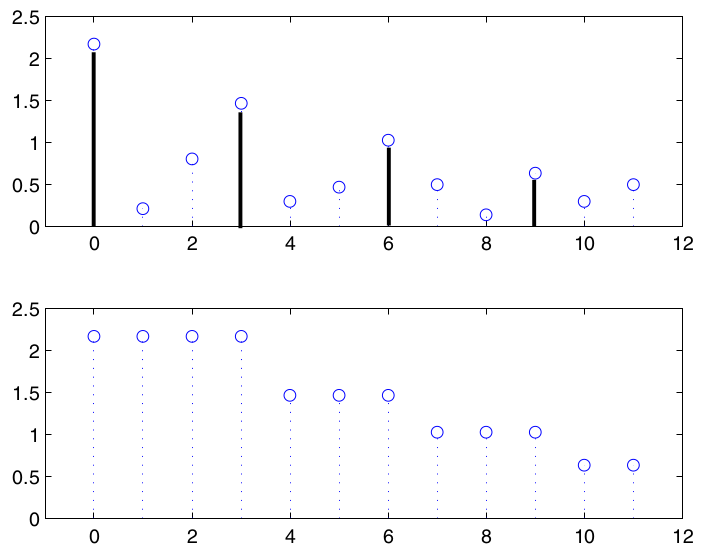
\includegraphics[width=0.5\linewidth]{nonmonotone}
	\caption{The sequences $\{f(x_k)\}_k$ and $\{R_k\}_k$.}
\end{figure}
\begin{theorem}
	Let $f\in \LC(\Rn)$ be limited from below. Let $\{x_k\}_k$ be a sequence generated by Algorithm \ref{alg:gd_armijo} with \eqref{eq:grippo} used in Algorithm \ref{alg:armijo} (instead of \eqref{eq:armijo}) for solving $\min_{x\in\Rn}\;f(x)$. Then we have 
	\begin{itemize}
		\item[(a)] $x_k \in \mathcal{L}_0 \;\;\forall k$ (where $\mathcal{L}_0:=\{x\in\Rn: f(x)\leq f(x_0)\}$)
		\item[(b)] $\displaystyle\lim_{k \to \infty} R_k = \displaystyle\lim_{k \to \infty} f(x_k) = f^*$ 
		\item[(c)] $\displaystyle\lim_{k \to \infty} \|\grad(x_k)\| = 0.$
	\end{itemize}
\end{theorem}
\begin{proof}
	First, we show that the sequence $\{R_k\}_k$ is monotonically nonincreasing. For each $k,$ let \\
	$r(k)\in[k-\min\{k,M\}, k]$ be the smallest integer such that 
\begin{equation*}
	R_k = f(x_{r(k)})=\max_{0\leq j \leq \min\{k,M\}} f(x_{k-j}).
\end{equation*}
Thus, we rewrite \eqref{eq:armijo} as
	\begin{equation}\label{eq:lemma_condition}
		f(x_{k+1}) \leq f(x_{r(k)}) - \alpha t_k \| \grad(x_k)\|^2 = f(x_{r(k)}) - \frac{\alpha}{t_k} \| x_{k+1} -x_k \|^2,
	\end{equation}
	Since min$(k+1, W) \leq $ min$(k, W) +1$, we have
	\begin{equation*}
		\begin{split}
			f(x_{r(k+1)}) &= \displaystyle \max_{0 \leq j \leq \text{min}(k+1, W)} f(x_{k-j+1})\\
			& \leq \displaystyle \max_{0 \leq j \leq \text{min}(k, W) +1} f(x_{k-j+1})\\
			& = \displaystyle \max \{ f(x_{r(k)}), f(x_{k+1})\} = f(x_{r(k)}),
		\end{split}
	\end{equation*}
	where last equality follows from (\ref{eq:lemma_condition}). Since $\{f(x_{r(k)})\}$ is nonincreasing and $x_{r(0)} = x_{0}$, we have that $f(x_k) \leq f(x^0) \; \forall k$, which proves $(a)$.
	\par Since $f$ is limited from below, the monotone nonincreasing sequence $\{f(x_{r(k)})\}$ admits a limit $f^*$ for $k \to \infty$. By induction on $j$, with $1\leq j \leq W+1$, let us prove that the two limits below are satisfied:
	\begin{eqnarray}
		\displaystyle \lim_{k \to \infty} \| x_{r(k) -j +1} -x_{r(k)-j}\| = 0 \label{eq:induction1}\\
		\displaystyle \lim_{k \to \infty} f(x_{r(k) -j}) = \displaystyle \lim_{k\to \infty} f(x_{r(k)}) \label{eq:induction2}
	\end{eqnarray}
	where $k$ is assumed to be large enough to have $r(k) \geq k -W >1.$
	\par If $j=1$, using $(\ref{eq:lemma_condition})$ with $k = r(k) - 1$, we have
	\begin{equation*}
		f(x_{r(k)}) \leq f(x_{r(r(k)-1)}) - \frac{\alpha}{t_{r(k)-1}}\| x_{r(k)} - x_{r(k)-1}\|^2.
	\end{equation*}
	Thus, together with convergence of $\{f(x_{r(k)})\}$ and the fact that $t_k\leq s$, we obtain 
	$$ \displaystyle \lim_{k \to \infty} \| x_{r(k)} -x_{r(k)-1}\| = 0$$
	From Lipschitz continuity of $f$ and the above limit we obtain that
	\begin{equation*}
		\displaystyle \lim_{k\to\infty} f(x_{r(k) -1}) = \displaystyle \lim_{k\to\infty} f(x_{r(k) }),
	\end{equation*}
	which means that induction has been proved for the case $j=1$.
	\par Now assume that (\ref{eq:induction1}) and (\ref{eq:induction2}) are valid for a given $j$. From (\ref{eq:lemma_condition}) used with\\ $k = r(k) -j -1$, we have that
	$$ f(x_{r(k) -j}) \leq f(x_{r(r(k)-j -1)}) - \frac{\alpha}{t_{r(k)-j-1}}\| x_{r(k)-j} - x_{r(k)-j-1}\|^2.$$
	Thus, together with (\ref{eq:induction2}), where the left limit is used for the LHS and the right limit is used for the RHS and remembering that $k=  r(k) -j -1$, and that $t_k\leq s$ we obtain that
	$$ \displaystyle \lim_{k \to \infty} \| x_{r(k)-j} - x_{r(k)-j-1} \| = 0.$$ 
	From the limit above, Lipschitz continuity of $f$ and again (\ref{eq:induction2}) we obtain that
	\begin{equation*}
		\displaystyle \lim_{k\to\infty} f(x_{r(k)-j-1}) =\displaystyle \lim_{k\to\infty} f(x_{r(k)-j})  = \displaystyle \lim_{k\to\infty} f(x_{r(k)}), 
	\end{equation*}
	which means that induction has been proved from a generic $j$ to $j+1$.
	\par In particular (\ref{eq:induction1}) and (\ref{eq:induction2}) are also valid if we replace $r(k)$ with $R(k):=r(k+W+1)$. Now, for $k$ sufficiently large, we have that
	\begin{equation} \label{eq:xk_to_xRk}
		\begin{split}
			x_{R(k)} &= x_k + (x_{k+1} - x_k) + \dots +(x_{R(k)} - x_{R(k)-1})\\
			&= x_k + \sum_{j=1}^{R(k)-k} \left (x_{R(k) -j +1} - x_{R(k)-j} \right ) 
		\end{split}
	\end{equation}
	Since $r(k+W+1) \leq k + W +1$, we have $R(k) -k  \leq W +1$ and, thus, from (\ref{eq:xk_to_xRk}) and (\ref{eq:induction1}) used replacing $r(k)$ with $R(k)$, we obtain 
	\begin{equation*}
		\displaystyle \lim_{k\to \infty} \| x_k - x_{R(k)}\| = 0.
	\end{equation*}
	From convergence of $\{f(x_{r(k)})\}$ and Lipschitz continuity, it follows that
	$$ \displaystyle\lim_{k\to \infty} f(x_k) = \displaystyle\lim_{k\to \infty}  f(x_{R(k)}) = \displaystyle\lim_{k\to \infty} f(x_{r(k+W+1)}) = f^*,$$
	which complete proof of $(b)$. Thesis $(c)$ follows from $(b)$, \eqref{eq:lemma_condition} and the fact that $t_k \geq \min\left \{s, \frac{2(1-\alpha)\beta}{L}\right \}$. 
\end{proof}

\subsection{Barzilai-Borwein Method}
%\subsubsection{The Quadratic Case}
Let us first consider a quadratic objective function, 
\begin{equation}\label{eq:quadratic}
	f(x) = x^TQx + c^Tx + b,
\end{equation}
where $x,c\in\Rn$, $b\in \R$, $Q\in \Rnn$ is symmetric and positive definite. In this case, we get the following result for GD.
\begin{proposition}[Finite convergence of GD in the quadratic case]
	Let $\lambda_1\geq \lambda_2, \dots,\lambda_n$ be the eigenvalue of the Hessian of the quadratic function \eqref{eq:quadratic}. Then, GD defined by the iteration
	\begin{equation}\label{eq:eigengrad}
		x_{k+1} = x_k -\frac{1}{\lambda_k} \grad(x_k) \quad \with k=1, \dots, n,
	\end{equation}
	determines in at maximum $n$ iterations the minimizer of $x_k$. 
\end{proposition}
\begin{proof}
	As gradient of \eqref{eq:quadratic} is $\grad(x)=Qx+c$, we get
	\begin{equation*}
		\grad(x_{k+1}) = Qx_{k+1} +c = Qx_k +c -\frac{1}{\lambda_k} Q \grad(x_k) = \left(I -\frac{1}{\lambda_k}Q\right)\grad(x_k)
	\end{equation*}
Repeating the application of the above formula, we get 
\begin{equation*}
	\grad(x_k) = \left(\prod_{j=1}^{k-1}(I-\frac{1}{\lambda_j}Q)\right)\grad(x_1)
\end{equation*}
Let ${u_h \in \Rn: h=1, \dots, n}$ be the set of eigenvectors of $Q$, associated to the eigenvalues $\lambda_h$, in particular they form a basis of $\Rn$, meaning that we can represent $\grad(x_1)$ as a linear combination of these vectors, i.e.,  
\begin{equation*}
	\grad(x_1) = \sum_{h=1}^{n} \beta_h u_h,\quad\with \beta_h\in\R. 
\end{equation*}
Thus, for $k\geq 2$, we get 
\begin{equation*}
	\grad(x_k) = \left(\prod_{j=1}^{k-1}(I-\frac{1}{\lambda_j}Q)\right) \left(\sum_{h=1}^{n} \beta_h u_h\right),
\end{equation*}
and consequently, setting $k=n+1$, from $Iu_h = u_h$ and $Qu_h=\lambda_hu_h$, we have
\begin{equation*}
	\grad(x_{n+1}) = \sum_{h=1}^{n} \beta_h \left(\prod_{j=1}^{n}(1-\frac{1}{\lambda_j}\lambda_h)\right) u_h=0,
\end{equation*}
from which we get that GD converges in at most $n$ steps.
\end{proof}
Unfortunately, the eigenvalues of $Q$ are usually not available and obtaining them is roughly as expensive as applying $GD$ on \eqref{eq:quadratic}. For this reason we consider instead of \eqref{eq:eigengrad} to approximate them on the fly via the Rayleigh quotient
\begin{equation*}
	R_Q(x) := \frac{x^TQx}{||x||^2} \quad \forall x\neq 0,
\end{equation*}
given that 
\begin{equation*}
	\lambda_n(Q) \leq R_Q(x) \leq \lambda_1(Q) \quad \with \forall x\neq 0. 
\end{equation*}
In particular, if the image of $Q$ is small (i.e., the interval $[\lambda_n(Q),\lambda_1(Q)]$ is small), $R_Q(x)$ approximates the eigenvalues of $Q$. Moreover, we can compute $R_Q(x)$ without 

\bibliographystyle{plain}
\bibliography{../biblio}
\end{document}